\chapter{Future Work} \label{future}

\section{Overview}
With the first official version of LIFE complete, updates and changes for a potential future version of LIFE is now examined. Having seen the results of the thermal-mechanical design in comparison with the simulated model, as well as examining the measured data, will give insights into how the instrument can be improved for the next flight, should an opportunity arise. Changes to the thermal-mechanical design is discussed first, if there were less constraints on the time and budget of the design. Second, the MCT characterization is reexamined. This section discusses what other tests could be completed with the detector, and any issues with the detector that arose. Finally, a discussion on the atmospheric instrument thermal model is presented, and what needs to be improved. 

\section{LIFE Thermal-Mechanical Design Changes}
The first version of LIFE had a number of constraints that led to the instrument being designed and built as it is. In future versions of the instrument, this may not be the case. A few changes to the instrument are examined here that could happen should another version of LIFE be approved, and incremental changes could be made. These changes aim to fix a few of the initial issues of the instrument, and also to make it easier to design, develop, and build. In addition these changes could help to provide better measurements and also better data analysis post-flight.

The first component that was planned to be fully updated in the next version of LIFE was the blackbody system. High-quality blackbody systems, as are needed for the calibration of highly sensitive thermal imaging systems, are expensive. This is why LIFE retrofitted an older blackbody system taken from a previous instrument. While the one used on LIFE was a high-quality system in terms of the blackbodies themselves, it did not fully suit the needs of LIFE. There are a number of changes that would be made and design requirements for a new blackbody system that should be considered if a system is designed or purchased for a future instrument. A few of the issues with the current system that would be changed are described here.

An issue with the blackbody system that was used for LIFE was the size and weight. Having been used in an instrument that required two full systems, it was large and heavy, and required the entire optical system to be raised so the window of the system would be aligned with the FTS. The bottom system was not used, and was unnecessary weight on an already heavy and bulky instrument, even with the unnecessary blackbodies removed. Some issues with the core mirror system also had to be dealt with, as the lack of encoder on the stepper motor as well as its age led to errors in the pointing of the mirror that may have caused self-emission issues. Finally, a general lack of information about the system due to its age led to some issues in the mechanical design. The system had to be measured and recreated in SolidWorks, and errors in this model led to some manufacturing errors that needed to be corrected. Other missing information included the surface coating of the mirror, which would have helped in determining self-emission, and there was little information given on the electrical system. A new blackbody system would be able to solve these issues, by making it smaller and designing it with the rest of the instrument in mind, as well as having information that was not available with the current system. A new and more precise centre motor system could also be installed to remove any viewing angle errors.

In addition to these issues and potential fixes to the blackbody system, an important component that was missing was the lack of a deep space view. Ideally, during flight and also just for characterization on the ground, the instrument would be able to view vertically upwards to space. This would provide another cold characterization point that would be colder than any blackbody or atmospheric view. Images of this cold view would be very helpful in the post-flight analysis of the data and would assist in self-emission and non-linearity removal methods. A basic mirror system was developed for the purpose of taking deep space measurements while performing instrument testing on the ground, which provided helpful data. A similar system could be implemented on a future flight instrument. An image of the temporary setup used for ground testing is shown in Figure \ref{fig:deepspace_mirror}. A better way to view a very cold blackbody, such as the blackbody used in the non-linearity characterization in the TVAC tank, could be combined with this new view to further improve characterization and post-flight analysis.

\begin{figure}
    \centering
    \rotatebox[origin=c]{270}{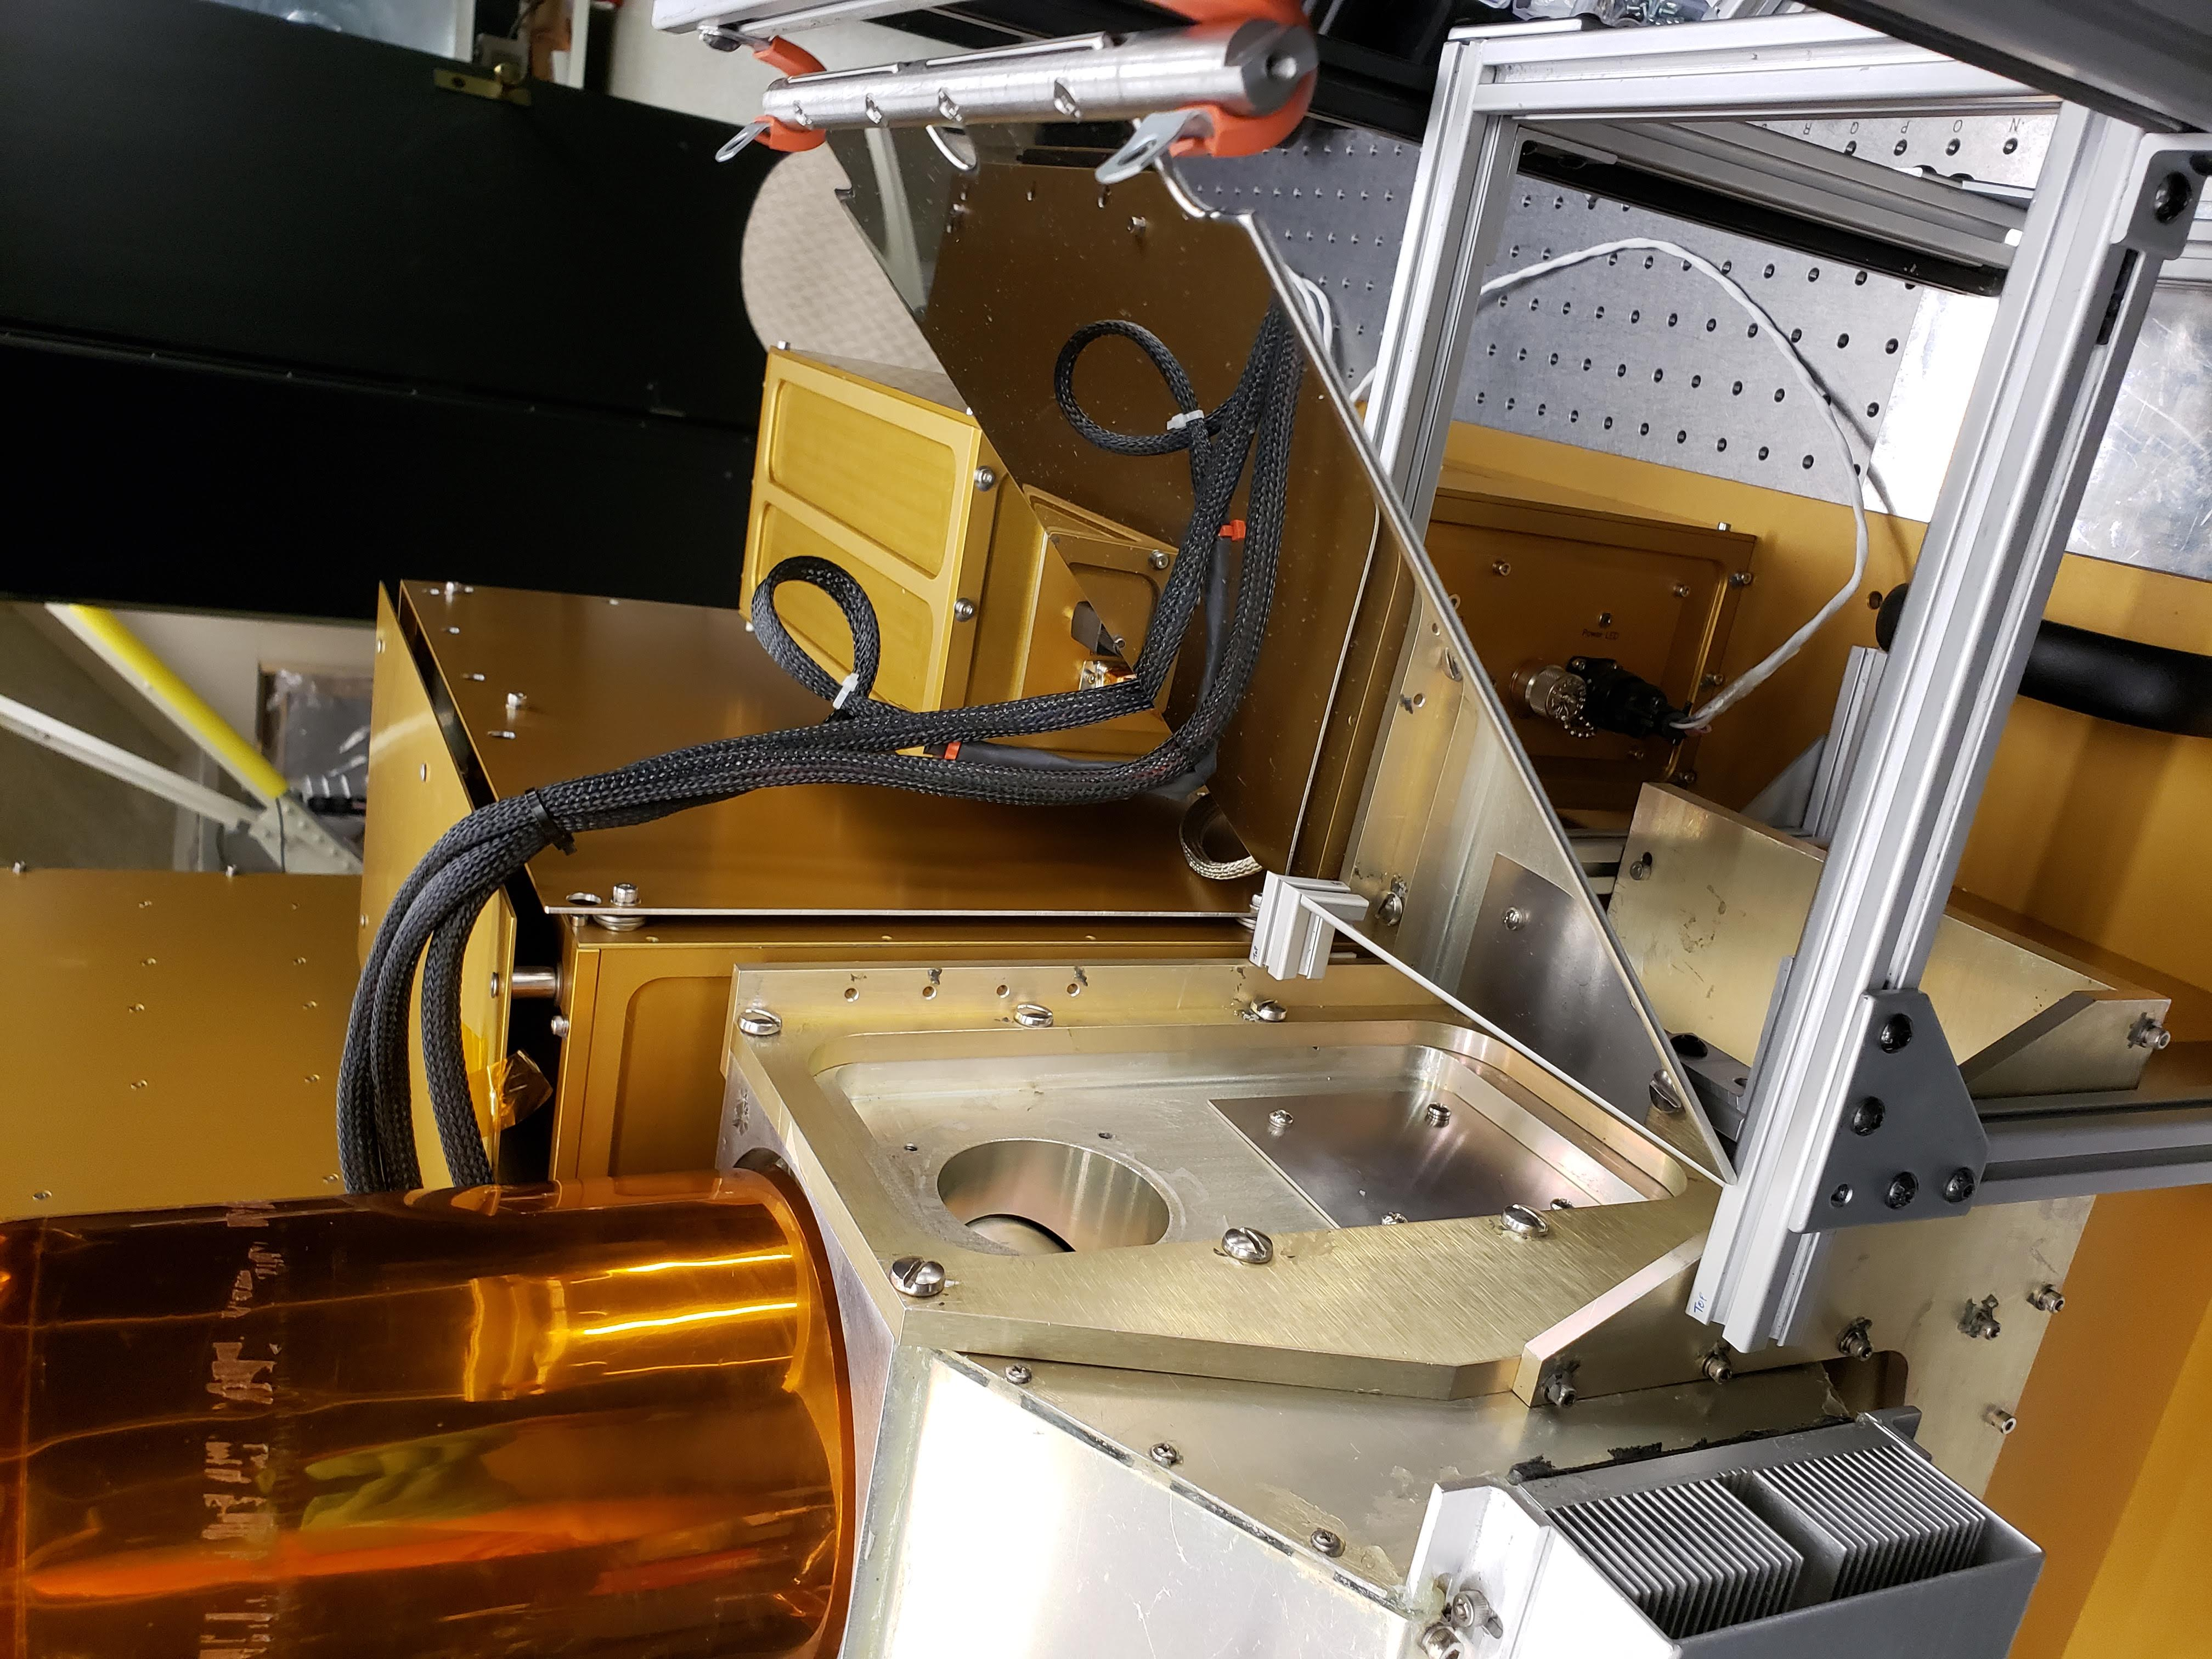
\includegraphics[width=0.7\linewidth]{other_images/LIFE_deepspace_viewing_mirror.jpg}}
    \caption{Mirror system for viewing vertically upwards towards space, for ground testing.}
    \label{fig:deepspace_mirror}
\end{figure}

Now looking beyond the blackbody, one of the design constraints that led to a much more complex design was the MCT detector orientation. With the pixels in a 1x16 horizontal array on the detector but a vertical field of view needed, the optical system needed to be mounted vertically. This led to increased complexity in the optical system design, and also led to difficulties with aligning and repairing the optical system as needed in this orientation. If a new MCT detector could be sourced, a detector with a vertical pixel array should be chosen. This would allow the optical system to be mounted horizontally and would be easier to test and align, as well as remain more stable during transport and flight. The remainder of the system could still stay the same, with the optical system being mounted to a breadboard and the system being thermally isolated still being design options with a horizontal optical system. The core optical system had issues with the field of view, which caused self emission errors, so this could be redesigned. However a more detailed discussion of an optical redesign is outside the scope of this thesis.

For more general mechanical updates, as mentioned briefly in Section \ref{construction_sec}, anodization should be considered more carefully, and it should be looked into if it could be applied to only specific areas. The anodization caused issues with the grounding of electronics, and needed to be removed in some areas so that electronics would have a direct electrical path to the box, which was also connected to the baseplate, which was used as the ground. If possible, small areas where electronics are mounted would not have anodization applied, so that is would not need to be removed later. This would be similar to the process of taping over a small area if the box was being painted, so that upon removal the surface would still be unpainted. In addition, an effort should be made to chose more uniform bolts, both for the cost of purchasing a large variety of bolts and so that it is easier to construct.

Finally, the instrument could be made to fly in daylight without much added cost or time. It is unknown how much lower temperatures would have been with the added sun shields used for daylight flights of the gondola, but likely a good amount. The addition of radiation panels to sensitive areas of the electronics boxes, such as the top part of the Electronics Box, would decrease the amount of solar heating from direct sunlight on these components. The effect of these radiation plates is evident in the low temperatures of the Optics Box even after sunrise. However, the dissipation of heat from the more powerful components of the Electronics Box may still cause issues. Methods for mitigating this may be performing more simulations with a painted rather than anodized box, which would allow more heat dissipation, or by adding a thermal path via copper strap from these components to the base of the instrument. More simulations need to be completed to examine possible thermal designs, but based on what was seen for the flight of the current instrument, daylight flight would likely be an option with a slightly modified design.

With most of these proposed changes to the thermal-mechanical design, a thorough redesign and rebuild of most of the instrument would be necessary. There are not many small incremental updates that could be done to the main instrument. Repairs need to be done to the current instrument, including reattaching the boxes to the baseplate properly, fixing the detector, and examining the optical system. However with a thorough update for a second version, especially with a new blackbody system, LIFE could be improved greatly for better measurements on future flights.

\section{Further MCT Characterization}
From the work that was completed on the detector prior to flight, the instrument performed well and took good measurements. The responsivity chosen limited the non-linearity seen, and the detector avoided saturation, so the settings chosen were good. However, further work could have been done to allow the detector to work better, which was not able to be completed. Beyond the verification and responsivity described in Chapter \ref{detector}, other characteristics of the detector were planned to be tested. Unfortunately nothing beyond the responsivity could be tested prior to flight, due to other testing and electrical issues until the launch that delayed any further testing. This was then planned to be completed post-launch, but as the detector was damaged during flight, this was not possible either. Here, a few detector characteristics that need further testing are described, if the detector is repaired for a future flight.

The responsivity and characterization done prior to flight should be further verified. There is no direct way to do this, as the characterization was done by changing the detector settings and examining the effect. After the settings were optimized, they were not changed afterwards, and were kept the same throughout the flight. A measure of the quality of the measurements is the non-linearity and Johnson noise of the data, which can be examined. The non-linearity was optimized for the settings chosen, but can be examined for the flight data to see if it was really minimized, or if better settings could have been chosen. Johnson noise is another method of examining this, and is connected to the non-linearity. However, an examination of both of these characteristics of the data requires a large amount of data analysis, and is outside the scope of this thesis. Both of these should be examined in the future to determine if the MCT should be further characterized and optimized.

As a whole, more work should be done into the characterization of the non-linearity. The original approach to correcting non-linearity was based on a three-point blackbody correction, following a method developed by the GLORIA team. For LIFE, a very cold blackbody in the TVAC tank was used, along with the warm and hot blackbodies, allowing three points of reference for correction. However, it was discovered that there was still a non-linearity that could not be corrected using this method, that was also found by GLORIA. It is a result in the strength of blackbody measurements versus deep space or limb measurements, causing inconsistencies~\citep{GLORIA_nonlinearity_PhD}. To correct for this, more points of measurement must be taken with blackbodies. Before future flights, measurements should be taken at a number of blackbody temperatures, in the ranges of cold, warm and hot, that can be used to create more points of correction. The issue of non-linearity is a well known problem with MCT detectors, and the majority of remaining characterization of the detector involves the non-linearity, and its minimization and removal from the data.

\section{Updates to Atmospheric Instrument Flight Thermal Model}
As discussed in Section \ref{flight_temp_model}, there were many unknowns in the post-flight detailed simulations that were deduced through a combination through known values and trial and error. While the model in the end was able to accurately match what was seen during flight, there is likely errors in the values chosen and they could be tweaked to more closely match what was actually seen. However, to do this, more temperature data is needed. This section will describe what parts of the thermal model could be improved through more instruments gathering data and improving the model with these measurements.

The ascent portion of the flight is the part of the model that has the largest room for error. Particularly as a result of convection, there are a large number of unknowns that are iterated through to be able to create an accurate temperature model. Ideally, more convection information is known about an ascent through this part of the atmosphere, but that is more complex to gather. What is more likely is that further instruments gather temperature data through this part of the flight, and apply the current values of convection to the new thermal model, and see how the temperatures match what was found during flight. Both the convection properties and the radiation properties may need to be altered to allow the temperatures to be match correctly, but the original values will serve as a starting point for the new model. Although they may not be accurate, the properties for convection and radiation should be close to what is needed for the new model and through a number of instruments these properties will converge and can provide information for future instruments better and faster. 

Similarly for the sunrise part of the flight, more information needs to be gathered on the affect of the sun on instruments of this altitude. The heat flux was included in the final part of the simulation and led to accurate temperatures, but there is little information known on how the sun was shining on the gondola. If possible it would be ideal to know this information for future daylight post-flight simulations, as it will allow more information for the thermal model. A longer time period of temperature measurements while the sun is shining on the gondola will provide this information.

The next instrument in the ISAS Atmospheric Research Group is currently being developed, and a full thermal model similar to LIFE is being developed for the flight. Although the instruments are different, the thermal model developed for LIFE will be able to inform some properties of the new simulations, and at the least provide good information on the environment. This will allow pre-flight simulations to go beyond the float portion of the flight and help to ensure better survivability.

\section{Conclusion}
The purpose of this thesis was to develop and prepare the LIFE instrument for an atmospheric balloon flight, where it would take measurements of greenhouse gases in the troposphere and stratosphere. A thermal-mechanical model of the instrument was developed, so that the instrument would be able to fly on a high-altitude balloon gondola, and be able to survive the environment of the flight. In addition, a core component of the instrument, the MCT detector, needed to be verified and characterized to ensure that it would operate and take good measurements during its flight.

Through 2018 and 2019, a model of LIFE was designed, developed, simulated, and built. It was flown at end of summer of 2019 on a gondola in Timmins, Ontario, to take measurements of the atmosphere and show that the instrument worked as expected. The flight was a success, all requirements of the thermal-mechanical design were met and the instrument took good measurements. Afterwards, from the data that was collected, a first iteration of a generalized thermal model for atmospheric instruments was developed, that could be used for future instruments as a starting point in the thermal design to save time and cost.

The purpose of creating the atmospheric balloon version of LIFE is to demonstrate that it can successfully operate and gather data on gases in the atmosphere. Information gathered from this flight, both its measurements and its operation, are used to inform future versions of LIFE, and eventually a satellite-borne instrument. 